
%% bare_conf.tex
%% V1.4b
%% 2015/08/26
%% by Michael Shell
%% See:
%% http://www.michaelshell.org/
%% for current contact information.
%%
%% This is a skeleton file demonstrating the use of IEEEtran.cls
%% (requires IEEEtran.cls version 1.8b or later) with an IEEE
%% conference paper.
%%
%% Support sites:
%% http://www.michaelshell.org/tex/ieeetran/
%% http://www.ctan.org/pkg/ieeetran
%% and
%% http://www.ieee.org/

%%*************************************************************************
%% Legal Notice:
%% This code is offered as-is without any warranty either expressed or
%% implied; without even the implied warranty of MERCHANTABILITY or
%% FITNESS FOR A PARTICULAR PURPOSE!
%% User assumes all risk.
%% In no event shall the IEEE or any contributor to this code be liable for
%% any damages or losses, including, but not limited to, incidental,
%% consequential, or any other damages, resulting from the use or misuse
%% of any information contained here.
%%
%% All comments are the opinions of their respective authors and are not
%% necessarily endorsed by the IEEE.
%%
%% This work is distributed under the LaTeX Project Public License (LPPL)
%% ( http://www.latex-project.org/ ) version 1.3, and may be freely used,
%% distributed and modified. A copy of the LPPL, version 1.3, is included
%% in the base LaTeX documentation of all distributions of LaTeX released
%% 2003/12/01 or later.
%% Retain all contribution notices and credits.
%% ** Modified files should be clearly indicated as such, including  **
%% ** renaming them and changing author support contact information. **
%%*************************************************************************


% *** Authors should verify (and, if needed, correct) their LaTeX system  ***
% *** with the testflow diagnostic prior to trusting their LaTeX platform ***
% *** with production work. The IEEE's font choices and paper sizes can   ***
% *** trigger bugs that do not appear when using other class files.       ***                          ***
% The testflow support page is at:
% http://www.michaelshell.org/tex/testflow/



\documentclass[conference]{IEEEtran}
% Some Computer Society conferences also require the compsoc mode option,
% but others use the standard conference format.
%
% If IEEEtran.cls has not been installed into the LaTeX system files,
% manually specify the path to it like:
% \documentclass[conference]{../sty/IEEEtran}





% Some very useful LaTeX packages include:
% (uncomment the ones you want to load)


% *** MISC UTILITY PACKAGES ***
%
%\usepackage{ifpdf}
% Heiko Oberdiek's ifpdf.sty is very useful if you need conditional
% compilation based on whether the output is pdf or dvi.
% usage:
% \ifpdf
%   % pdf code
% \else
%   % dvi code
% \fi
% The latest version of ifpdf.sty can be obtained from:
% http://www.ctan.org/pkg/ifpdf
% Also, note that IEEEtran.cls V1.7 and later provides a builtin
% \ifCLASSINFOpdf conditional that works the same way.
% When switching from latex to pdflatex and vice-versa, the compiler may
% have to be run twice to clear warning/error messages.






% *** CITATION PACKAGES ***
%
%\usepackage{cite}
% cite.sty was written by Donald Arseneau
% V1.6 and later of IEEEtran pre-defines the format of the cite.sty package
% \cite{} output to follow that of the IEEE. Loading the cite package will
% result in citation numbers being automatically sorted and properly
% "compressed/ranged". e.g., [1], [9], [2], [7], [5], [6] without using
% cite.sty will become [1], [2], [5]--[7], [9] using cite.sty. cite.sty's
% \cite will automatically add leading space, if needed. Use cite.sty's
% noadjust option (cite.sty V3.8 and later) if you want to turn this off
% such as if a citation ever needs to be enclosed in parenthesis.
% cite.sty is already installed on most LaTeX systems. Be sure and use
% version 5.0 (2009-03-20) and later if using hyperref.sty.
% The latest version can be obtained at:
% http://www.ctan.org/pkg/cite
% The documentation is contained in the cite.sty file itself.






% *** GRAPHICS RELATED PACKAGES ***
%
\ifCLASSINFOpdf
  \usepackage{listings}
  \usepackage[pdftex]{graphicx}
  \usepackage{url}

  % declare the path(s) where your graphic files are
  % \graphicspath{{../pdf/}{../jpeg/}}
  % and their extensions so you won't have to specify these with
  % every instance of \includegraphics
  % \DeclareGraphicsExtensions{.pdf,.jpeg,.png}
\else
  % or other class option (dvipsone, dvipdf, if not using dvips). graphicx
  % will default to the driver specified in the system graphics.cfg if no
  % driver is specified.
  % \usepackage[dvips]{graphicx}
  % declare the path(s) where your graphic files are
  % \graphicspath{{../eps/}}
  % and their extensions so you won't have to specify these with
  % every instance of \includegraphics
  % \DeclareGraphicsExtensions{.eps}
\fi
% graphicx was written by David Carlisle and Sebastian Rahtz. It is
% required if you want graphics, photos, etc. graphicx.sty is already
% installed on most LaTeX systems. The latest version and documentation
% can be obtained at:
% http://www.ctan.org/pkg/graphicx
% Another good source of documentation is "Using Imported Graphics in
% LaTeX2e" by Keith Reckdahl which can be found at:
% http://www.ctan.org/pkg/epslatex
%
% latex, and pdflatex in dvi mode, support graphics in encapsulated
% postscript (.eps) format. pdflatex in pdf mode supports graphics
% in .pdf, .jpeg, .png and .mps (metapost) formats. Users should ensure
% that all non-photo figures use a vector format (.eps, .pdf, .mps) and
% not a bitmapped formats (.jpeg, .png). The IEEE frowns on bitmapped formats
% which can result in "jaggedy"/blurry rendering of lines and letters as
% well as large increases in file sizes.
%
% You can find documentation about the pdfTeX application at:
% http://www.tug.org/applications/pdftex





% *** MATH PACKAGES ***
%
%\usepackage{amsmath}
% A popular package from the American Mathematical Society that provides
% many useful and powerful commands for dealing with mathematics.
%
% Note that the amsmath package sets \interdisplaylinepenalty to 10000
% thus preventing page breaks from occurring within multiline equations. Use:
%\interdisplaylinepenalty=2500
% after loading amsmath to restore such page breaks as IEEEtran.cls normally
% does. amsmath.sty is already installed on most LaTeX systems. The latest
% version and documentation can be obtained at:
% http://www.ctan.org/pkg/amsmath





% *** SPECIALIZED LIST PACKAGES ***
%
%\usepackage{algorithmic}
% algorithmic.sty was written by Peter Williams and Rogerio Brito.
% This package provides an algorithmic environment fo describing algorithms.
% You can use the algorithmic environment in-text or within a figure
% environment to provide for a floating algorithm. Do NOT use the algorithm
% floating environment provided by algorithm.sty (by the same authors) or
% algorithm2e.sty (by Christophe Fiorio) as the IEEE does not use dedicated
% algorithm float types and packages that provide these will not provide
% correct IEEE style captions. The latest version and documentation of
% algorithmic.sty can be obtained at:
% http://www.ctan.org/pkg/algorithms
% Also of interest may be the (relatively newer and more customizable)
% algorithmicx.sty package by Szasz Janos:
% http://www.ctan.org/pkg/algorithmicx




% *** ALIGNMENT PACKAGES ***
%
%\usepackage{array}
% Frank Mittelbach's and David Carlisle's array.sty patches and improves
% the standard LaTeX2e array and tabular environments to provide better
% appearance and additional user controls. As the default LaTeX2e table
% generation code is lacking to the point of almost being broken with
% respect to the quality of the end results, all users are strongly
% advised to use an enhanced (at the very least that provided by array.sty)
% set of table tools. array.sty is already installed on most systems. The
% latest version and documentation can be obtained at:
% http://www.ctan.org/pkg/array


% IEEEtran contains the IEEEeqnarray family of commands that can be used to
% generate multiline equations as well as matrices, tables, etc., of high
% quality.




% *** SUBFIGURE PACKAGES ***
%\ifCLASSOPTIONcompsoc
%  \usepackage[caption=false,font=normalsize,labelfont=sf,textfont=sf]{subfig}
%\else
%  \usepackage[caption=false,font=footnotesize]{subfig}
%\fi
% subfig.sty, written by Steven Douglas Cochran, is the modern replacement
% for subfigure.sty, the latter of which is no longer maintained and is
% incompatible with some LaTeX packages including fixltx2e. However,
% subfig.sty requires and automatically loads Axel Sommerfeldt's caption.sty
% which will override IEEEtran.cls' handling of captions and this will result
% in non-IEEE style figure/table captions. To prevent this problem, be sure
% and invoke subfig.sty's "caption=false" package option (available since
% subfig.sty version 1.3, 2005/06/28) as this is will preserve IEEEtran.cls
% handling of captions.
% Note that the Computer Society format requires a larger sans serif font
% than the serif footnote size font used in traditional IEEE formatting
% and thus the need to invoke different subfig.sty package options depending
% on whether compsoc mode has been enabled.
%
% The latest version and documentation of subfig.sty can be obtained at:
% http://www.ctan.org/pkg/subfig




% *** FLOAT PACKAGES ***
%
%\usepackage{fixltx2e}
% fixltx2e, the successor to the earlier fix2col.sty, was written by
% Frank Mittelbach and David Carlisle. This package corrects a few problems
% in the LaTeX2e kernel, the most notable of which is that in current
% LaTeX2e releases, the ordering of single and double column floats is not
% guaranteed to be preserved. Thus, an unpatched LaTeX2e can allow a
% single column figure to be placed prior to an earlier double column
% figure.
% Be aware that LaTeX2e kernels dated 2015 and later have fixltx2e.sty's
% corrections already built into the system in which case a warning will
% be issued if an attempt is made to load fixltx2e.sty as it is no longer
% needed.
% The latest version and documentation can be found at:
% http://www.ctan.org/pkg/fixltx2e


%\usepackage{stfloats}
% stfloats.sty was written by Sigitas Tolusis. This package gives LaTeX2e
% the ability to do double column floats at the bottom of the page as well
% as the top. (e.g., "\begin{figure*}[!b]" is not normally possible in
% LaTeX2e). It also provides a command:
%\fnbelowfloat
% to enable the placement of footnotes below bottom floats (the standard
% LaTeX2e kernel puts them above bottom floats). This is an invasive package
% which rewrites many portions of the LaTeX2e float routines. It may not work
% with other packages that modify the LaTeX2e float routines. The latest
% version and documentation can be obtained at:
% http://www.ctan.org/pkg/stfloats
% Do not use the stfloats baselinefloat ability as the IEEE does not allow
% \baselineskip to stretch. Authors submitting work to the IEEE should note
% that the IEEE rarely uses double column equations and that authors should try
% to avoid such use. Do not be tempted to use the cuted.sty or midfloat.sty
% packages (also by Sigitas Tolusis) as the IEEE does not format its papers in
% such ways.
% Do not attempt to use stfloats with fixltx2e as they are incompatible.
% Instead, use Morten Hogholm'a dblfloatfix which combines the features
% of both fixltx2e and stfloats:
%
% \usepackage{dblfloatfix}
% The latest version can be found at:
% http://www.ctan.org/pkg/dblfloatfix




% *** PDF, URL AND HYPERLINK PACKAGES ***
%
%\usepackage{url}
% url.sty was written by Donald Arseneau. It provides better support for
% handling and breaking URLs. url.sty is already installed on most LaTeX
% systems. The latest version and documentation can be obtained at:
% http://www.ctan.org/pkg/url
% Basically, \url{my_url_here}.




% *** Do not adjust lengths that control margins, column widths, etc. ***
% *** Do not use packages that alter fonts (such as pslatex).         ***
% There should be no need to do such things with IEEEtran.cls V1.6 and later.
% (Unless specifically asked to do so by the journal or conference you plan
% to submit to, of course. )


% correct bad hyphenation here
\hyphenation{op-tical net-works semi-conduc-tor}


\begin{document}
%
% paper title
% Titles are generally capitalized except for words such as a, an, and, as,
% at, but, by, for, in, nor, of, on, or, the, to and up, which are usually
% not capitalized unless they are the first or last word of the title.
% Linebreaks \\ can be used within to get better formatting as desired.
% Do not put math or special symbols in the title.
\title{How Important are Usage Examples in REST API Documentation?}

% author names and affiliations
% use a multiple column layout for up to three different
% affiliations
\author{\IEEEauthorblockN{S M Sohan, Frank Maurer\IEEEauthorrefmark{1}}
\IEEEauthorblockA{\IEEEauthorrefmark{1}
Dept. of Computer Science\\
University of Calgary\\
Canada\\
\{smsohan, frank.maurer\}@ucalgary.ca}
\and
\IEEEauthorblockN{Craig Anslow}
\IEEEauthorblockA{School of Eng. and Computer Science\\
Victoria University of Wellington\\
New Zealand\\
craig@ecs.vuw.ac.nz}
\and
\IEEEauthorblockN{Martin Robillard}
\IEEEauthorblockA{
School of Computer Science\\
McGill University\\
Canada\\
martin@cs.mcgill.ca}
}

% conference papers do not typically use \thanks and this command
% is locked out in conference mode. If really needed, such as for
% the acknowledgment of grants, issue a \IEEEoverridecommandlockouts
% after \documentclass

% for over three affiliations, or if they all won't fit within the width
% of the page, use this alternative format:
%
%\author{\IEEEauthorblockN{Michael Shell\IEEEauthorrefmark{1},
%Homer Simpson\IEEEauthorrefmark{2},
%James Kirk\IEEEauthorrefmark{3},
%Montgomery Scott\IEEEauthorrefmark{3} and
%Eldon Tyrell\IEEEauthorrefmark{4}}
%\IEEEauthorblockA{\IEEEauthorrefmark{1}School of Electrical and Computer Engineering\\
%Georgia Institute of Technology,
%Atlanta, Georgia 30332--0250\\ Email: see http://www.michaelshell.org/contact.html}
%\IEEEauthorblockA{\IEEEauthorrefmark{2}Twentieth Century Fox, Springfield, USA\\
%Email: homer@thesimpsons.com}
%\IEEEauthorblockA{\IEEEauthorrefmark{3}Starfleet Academy, San Francisco, California 96678-2391\\
%Telephone: (800) 555--1212, Fax: (888) 555--1212}
%\IEEEauthorblockA{\IEEEauthorrefmark{4}Tyrell Inc., 123 Replicant Street, Los Angeles, California 90210--4321}}




% use for special paper notices
%\IEEEspecialpapernotice{(Invited Paper)}




% make the title area
\maketitle

% As a general rule, do not put math, special symbols or citations
% in the abstract
\begin{abstract}
\end{abstract}

% no keywords




% For peer review papers, you can put extra information on the cover
% page as needed:
% \ifCLASSOPTIONpeerreview
% \begin{center} \bfseries EDICS Category: 3-BBND \end{center}
% \fi
%
% For peerreview papers, this IEEEtran command inserts a page break and
% creates the second title. It will be ignored for other modes.
\IEEEpeerreviewmaketitle

\section{Introduction}
\section{Methodolody}
\subsection{Research Goals}

This research is aimed at answering the following research questions:

\begin{itemize}
  \item \textbf{RQ1}. What impact does usage examples have on REST API client developer productivity?
  \item \textbf{RQ2}. What problems API client developers face when using a REST API documentation that lacks usage examples?
\end{itemize}

\subsection{Requirements} % (fold)

To answer the aforementioned research questions, the study has the following requirements:

\begin{itemize}
  \item \textbf{R1. Realistic.} We had to choose an existing REST API that is currently used by API client developers. Selecting a mature REST API for this study reduces the possibility of an underdeveloped solution that may be found if a new or a seldom used API is selected. A familiar domain needed to be selected so that participants are able to relate to the API features without requiring upfront training. In addition to selecting the API, we had to select tasks that are related to the core features provided by the API to represent reality.
  \item \textbf{R2. Open source.} To be able to understand the impact of usage examples, we needed to select an open-source API where we can add new examples to the documentation for performing this study. For proprietary APIs, it won't be possible to retrofit usage examples on existing API documentation without separating the examples from the documentation.
  \item \textbf{R3. Time bound.} The total time spent by each participant is required to be time bound to measure productivity. As a result, the study needs to be setup such that participants are able to focus on performing the tasks minimizing any overhead.
  \item \textbf{R4. Experienced developers.} Developers with prior experience on REST APIs need to be recruited as study participants to perform the study within a limited amount of time and in a realistic setup. Furthermore, to reduce a learning bias, only participants with no prior experince of using the WordPress REST API V2 are accepted for this study.
\end{itemize}


\subsection{Study API} % (fold)

We selected the WordPress REST API V2 for this study. WordPress is a blog-like open-source (R2) framework used by over 409 million people to visit 23.6 billion pages each month. The API allows programmatic access to list, create, update, and delete WordPress data such as blog posts, comments, users, images, tags, etc.

The WordPress REST API V2 has been published and maintained since May 2015. Before January 2017, the WordPress REST API V2 was distributed as a plug-in where WordPress users could optionally install the API component. The following statistics are for the plug-in install numbers between May 2015 and October 2016:

\begin{itemize}
  \item Total installs: aprox. 248K installs of the plug-in.
  \item Average daily installs: approx. 500.
\end{itemize}

Starting January 2017, the WordPress REST API V2 is no longer required to be installed as a separate plug-in since it's pre-bundled with every WordPress install. As per the code repository on GitHub, there are a total of 99 and 46 contributors that had at least one commit to the code repository behind the API and and it's documentation, respectively. These properties satisfy R1, our requirements for being realistic.

By selecting an open-source project we are able to access the source-code to inspect the implementation and documentation technique of the WordPress REST API. The API implements a self-documenting feature where API developers expose API endpoints over HTTP OPTIONS verb to explain the API elements. To implement this feature, the API developers describe the API elements in the code. For example:


\lstset{basicstyle=\footnotesize}
\begin{lstlisting}[language=php,breaklines=true,showspaces=false,showstringspaces=false,numbers=left,xleftmargin=2em,caption={Example of self-documenting API Code},label=wordpress_code]
public function get_item_schema() {
  $schema = array(
    '$schema'    => 'http://json-schema.org/draft-04/schema#',
    'title'      => $this->post_type,
    'type'       => 'object',
    /*
     * Base properties for every Post.
     */
    'properties' => array(
        'date'            => array(
            'description' => __( "The date the object was published, in the site's timezone." ),
            'type'        => 'string',
            'format'      => 'date-time',
            'context'     => array( 'view', 'edit', 'embed' ),
        ),...
\end{lstlisting}

On Listing \ref{wordpress_code}, line 4 specifies that this is a schema definition for the API element $Post$. Then, on Line 10, it defines $date$, one of the properties of $Post$, followed by a human readable description and and type information. Then, on line 14, the context of this property is mentioned as $view, edit, embed$, meaning that this property will be returned when the $Post$ object is returned, embedded, or can be used as an input for editing.

This self-documenting feature is leveraged to generate and publish the official API documentation as an HTML website. Figure \ref{fig:schema} shows a screenshot of the published documentation for the $date$ attribute of the $Post$ API element\footnote{\url{http://v2.wp-api.org/reference/posts/}}.

\begin{figure}[h!]
\begin{center}
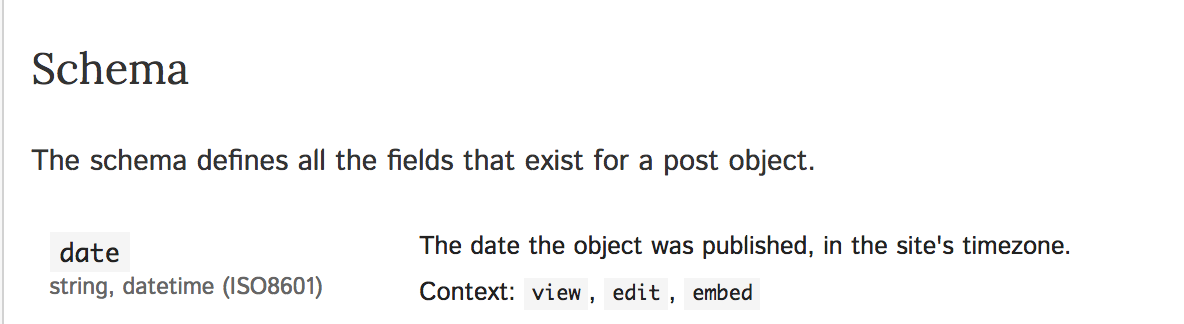
\includegraphics[width=\linewidth,keepaspectratio]{schema.png}
\end{center}
\caption{Screenshot showing auto-generated documentation for Post/date}
\label{fig:schema}
\end{figure}

In addition to the auto-generated documentation of the the schema and API actions, custom content is added by the contributors to the API documentation project to provide prosaic overviews and usage examples.



\subsection{Study Design} % (fold)
\subsubsection{Tasks} % (fold)

The participants are requested to perform a total of six tasks using the API including one practice task. All of the tasks are related to a single API element, $Post$. The tasks get progressively difficult, and all but the last task can be performed independently of each other. Participants are requested to limit the total time on the study to a maximum of one hour. Participants are encouraged to proceed to the next task when they are either satisfied about or stuck on the right answer.

To use a REST API, the API client developers need to work with the following four inputs over HTTP:

\begin{itemize}
  \item I1. Request method
  \item I2. Request URL
  \item I3. Request headers
  \item I4. Request body
\end{itemize}

To verify the response of an API call, the API client developers can use HTTP response headers and/or HTTP response body. To perform the tasks, the participants are required to use one or more of the inputs I1-4. In the following paragraphs, we describe each task with it's description and the intended test scenario against the aforementioned API input and output information. For each of the tasks, the participants are required to use the same WordPress REST API and its documentation.

\textbf{T1: ListAllPostsTask}. We ask the participants to use the WordPress REST API following its documentation to get a list of the blog posts from a live WordPress site. This is the practice task, and the inputs to answer this task are pre-filled for the participants. It allows the participants to understand the tools used for this study as well as get familiarity with the Post API. The answer for this task makes use of I1 and I2.

\textbf{T2: FilterPostsByAuthorTask.} The participants are asked to use the API to filter the list of posts by an author given the author's user name. To answer this correctly, the participants are required to first make an API call to get the numeric ID of the author given the string based user name. Then, the ID needs to be used on the Post API to filter posts by the author. This task allows us to understand the impact of usage examples on API client developers when multiple API calls need to be made to perform a task using the API. Inputs I1-2 are required to complete this task successfully.

\textbf{T3: ExcludePostsByIdsTask.} We ask the participants to use the API to get a list of all posts excluding posts with IDs 1 and 4. Participants need to use the inputs I1-2, and use a desired format on I2 to pass an array of IDs as a parameter. This task allows us to understand how API client developers identify the format for using an array within the URL with respect to the usage examples in the API documentation.

\textbf{T4: FindTotalPostsTasks.} This task requires the participants to use the API to find a total number of posts. Participants need to use the inputs I1-2 and inspect the HTTP response headers to successfully complete this task. This task allows us to understand how API client developer productivity is affected with respect to missing examples about HTTP response headers in the API documentation.

\textbf{T5: PublishPostTask.} We ask the participants to use the API to publish a blog post with a specific title, content, and a published date. To successfully complete this task, the participants are required to use all four input types and inspect both the HTTP response header and the response body. Additionally, the participants are required to use a specific date format that the API accepts as a valid format for date specification. Answers to this task allows us to study API client developer productivity with respect to the usage examples lacking details about the inputs I3-4.

\textbf{T6: UpdatePostTask.} We ask the participants to use the API to update a blog post that they published in T5 with a new excerpt. Similar to T5, this task requires the use of inputs I1-4, but with different values for the inputs. This task allows us to understand API client developer productivity on inter-dependent tasks with respect to usage examples.

To summarize, the tasks allow us to understand how REST API client developers approach API tasks of different complexity levels involving various input types and available output information with respect to the usage examples in the API documentation.

\subsubsection{Participant Selection} % (fold)

To satisfy the requirement of developers with REST API experience (R3), we have used the following criteria for recruiting the study participants:

\begin{itemize}
  \item Currently working as a software engineer.
  \item At least 1 year of industry experience as a software engineer.
  \item At least 1 year of industry experience with REST APIs.
  \item No prior experience with WordPress REST API.
\end{itemize}

Participants were recruited through online announcements posted on Twitter, Facebook, and software developer focused mailing lists.

\subsubsection{Process}

Two pilot studies were performed to evaluate and understand an effective process for performing this study. The first pilot study involved four participants that were invited to join the first author on this paper in-person or using a video conferencing software. The study involved tasks using two APIs, the WordPress REST API V2 and the GMail REST API. Each participant was given one of the two APIs and a set of tasks to complete using the API within an hour. Participants were given an online answer form to record the answers to the tasks. The primary findings from this pilot are as follows: 1) asking participants to use an API to perform the tasks required significant overhead time for them to setup a development environment with the proper API credentials, 2) the intermediate trial attempts of using the API are potentially more valuable than the final answer as it allows us to understand API client developer information needs that may are not answered by the documentation, 3) the number of tasks for the study had to be reduced so the participants could complete the tasks within the one hour limit, and 4) for GMail API, participants used up a large portion of their time on setting up their API credentials that requires understanding of OAuth.


\begin{figure*}[t]
\begin{center}
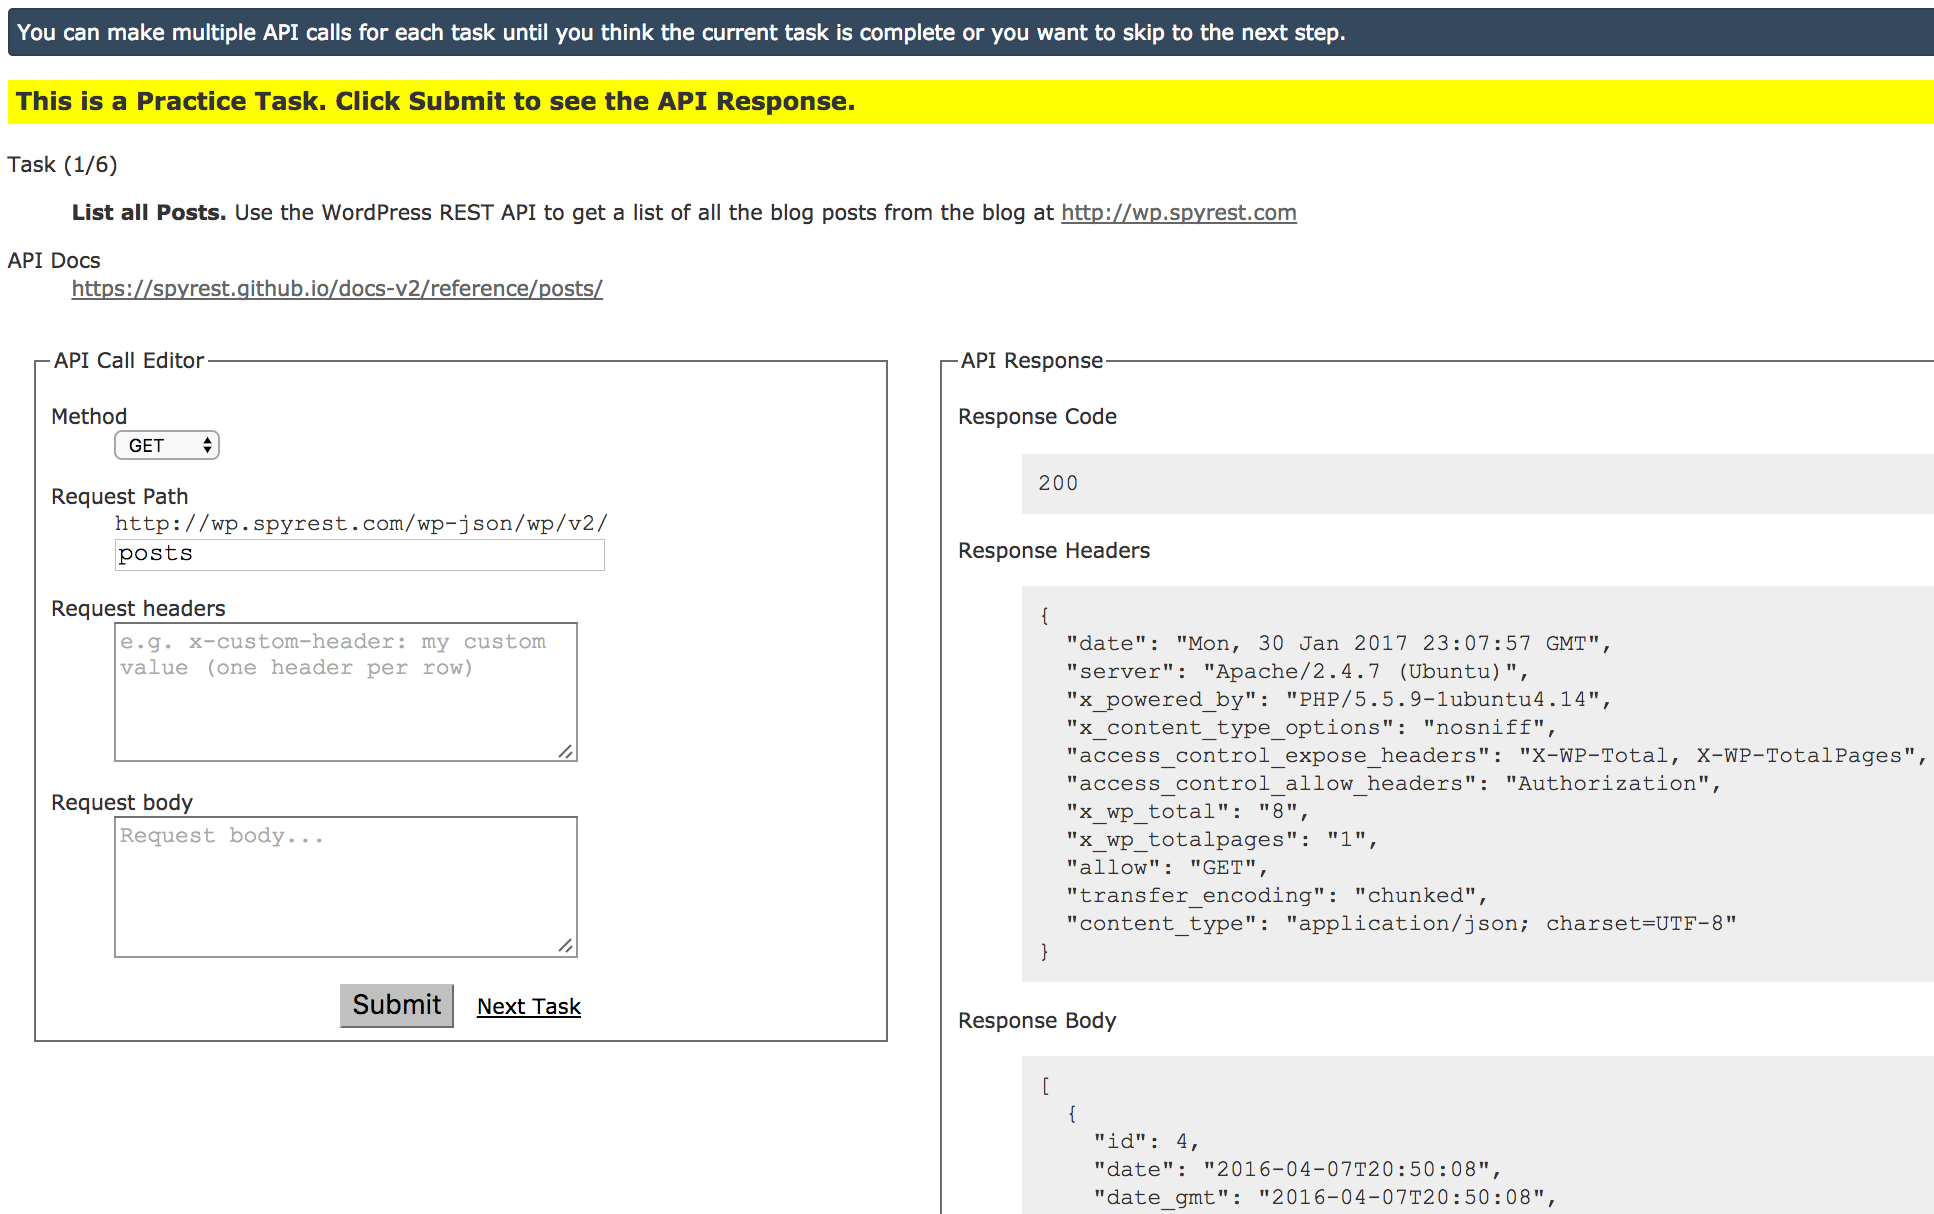
\includegraphics[width=\linewidth,keepaspectratio]{api_explorer.png}
\end{center}
\caption{Screenshot of the web-based REST API explorer}
\label{fig:api_explorer}
\end{figure*}

To overcome the shortcomings found from the first pilot study, we decided to develop a web-based REST API explorer as shown on Figure \ref{fig:api_explorer} that allows participants to use their browser to make the API calls without setting up any development environment. The web-based API explorer only requires the inputs I1-4, and displays the HTTP response headers and body on the click of a button. Thus the participants could focus on using the right input and verifying the output without having to write any code. The web-base REST API explorer also allowed us to automatically collect all the trial API calls that the participants make for each API task. A second pilot study involving seven new participants was performed to understand the features of the web-based REST API explorer in practice and to improve the user interface based on feedback from the participants. Participants completed the study on their own without having to meet in-person or over video conferencing. Only the WordPress REST API was used to focus on REST APIs without the required learning curve associated with OAuth. We found encouraging results from this pilot study as the collected data showed patterns of mistakes that API client developers make that can be reduced by adding usage examples in the API documentation.


\begin{figure*}[t]
\begin{center}
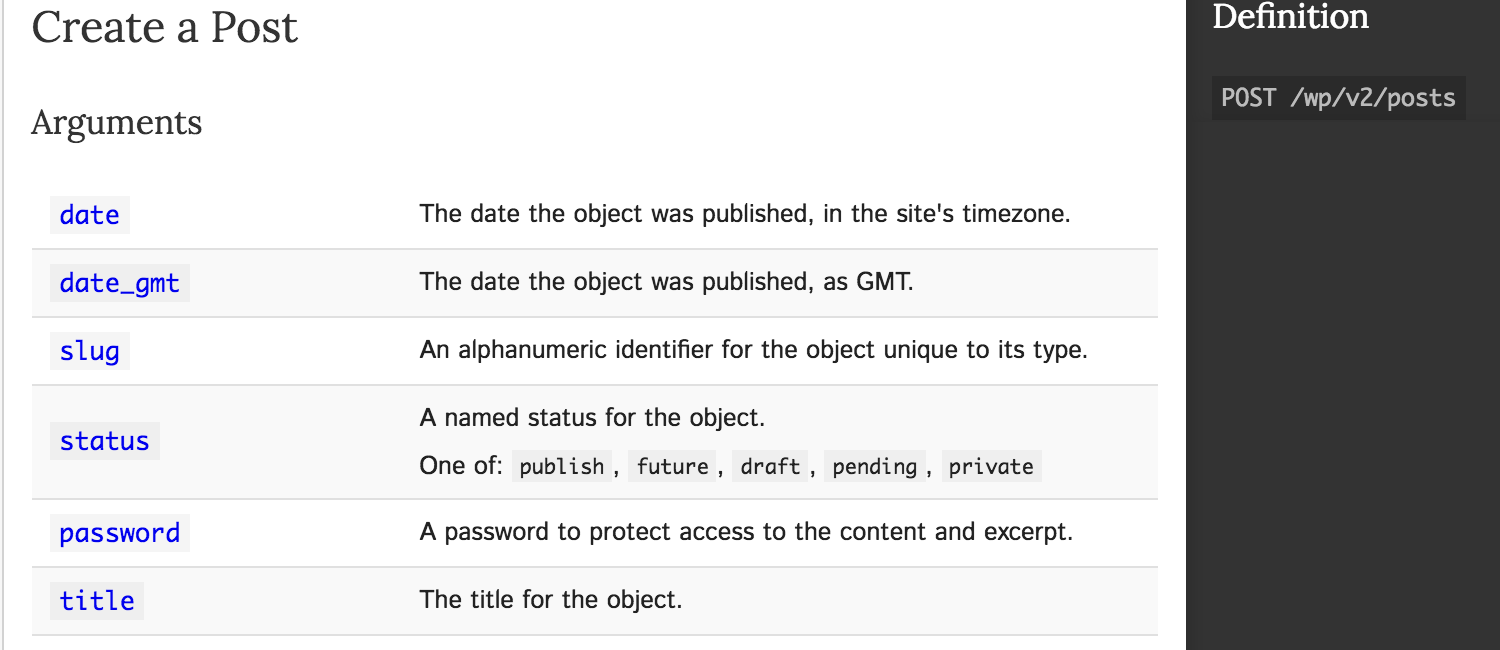
\includegraphics[width=\linewidth,keepaspectratio]{original.png}
\end{center}
\caption{Screenshot of the original WordPress REST API documentation}
\label{fig:original}
\end{figure*}

\begin{figure*}[tb]
\begin{center}
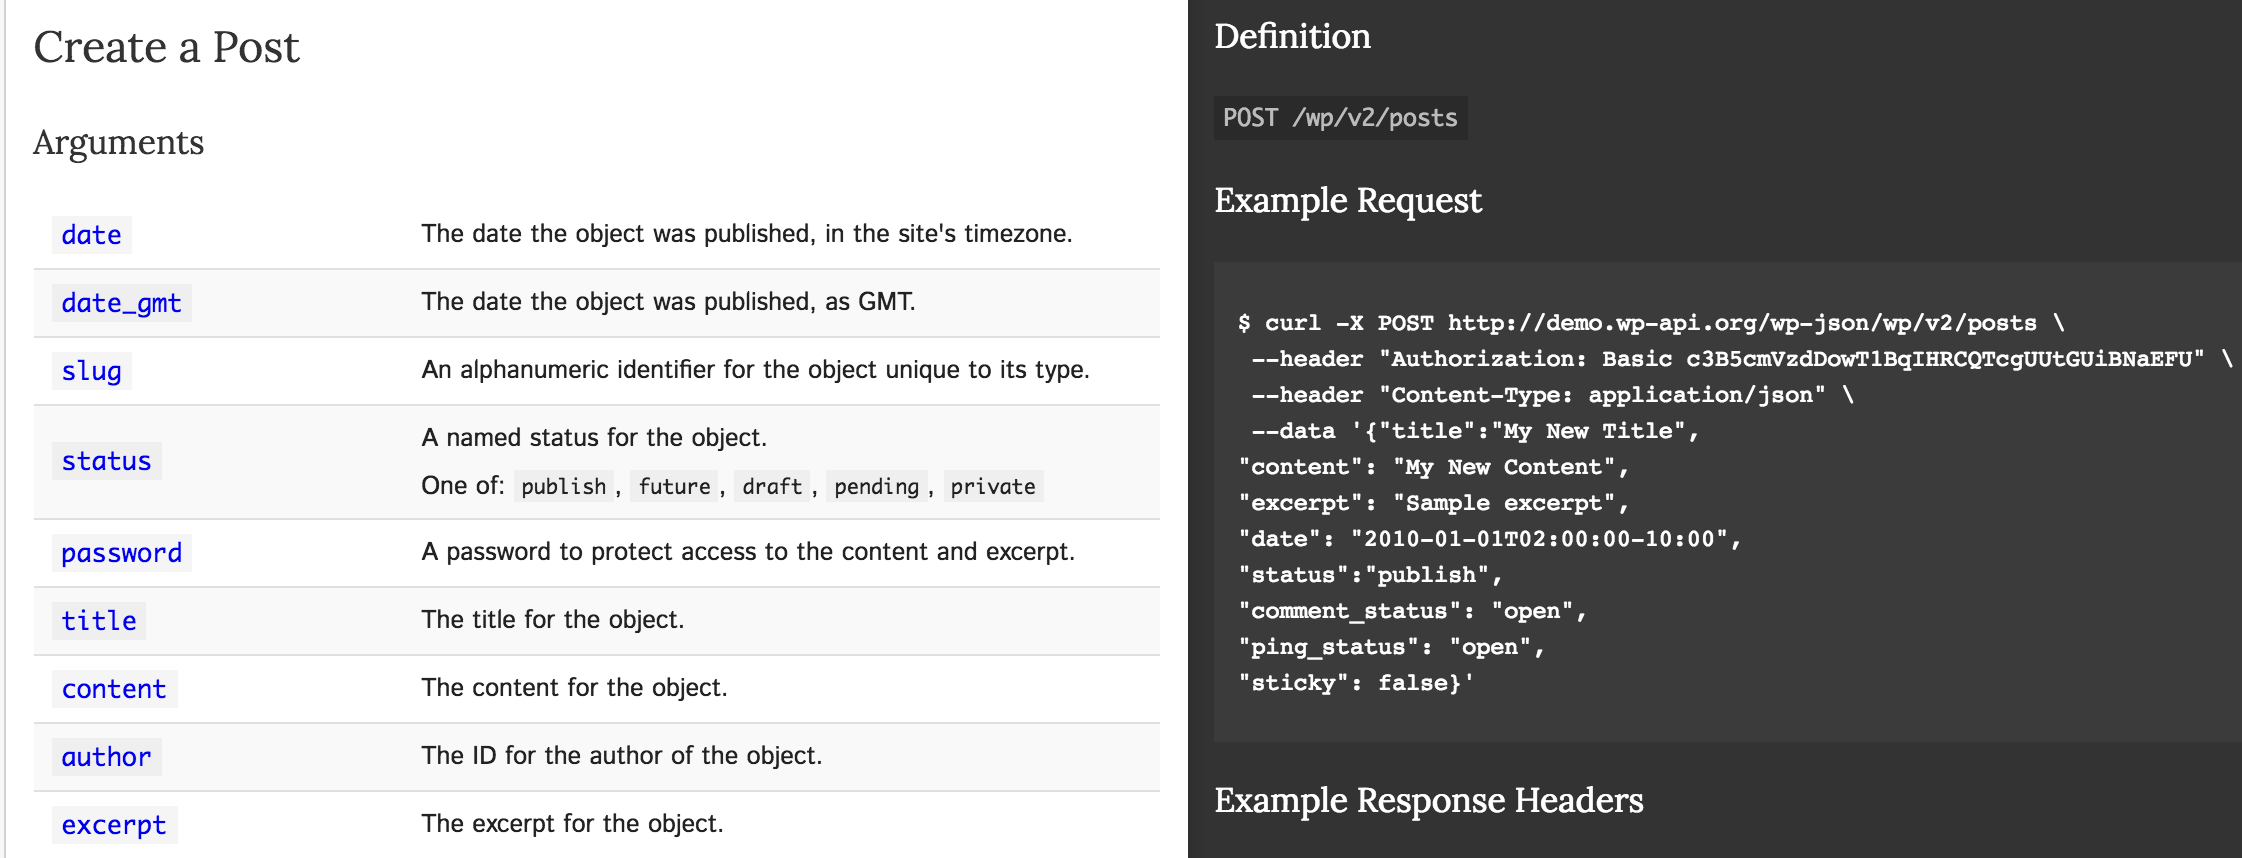
\includegraphics[width=\linewidth,keepaspectratio]{forked.png}
\end{center}
\caption{Screenshot of the forked WordPress REST API documentation with a usage example}
\label{fig:forked}
\end{figure*}


Based on the lessons learned from the pilot studies, we designed the actual study process as follows: the original WordPress REST API documentation was forked and a total of 3 API usage examples were added to show listing of blog posts with query parameters for filtering, a request to create a blog post and a request to update a blog post. Figure \ref{fig:original} shows a screenshot of the original API documentation related to T4 where the API client developers are provided with a reference table describing the different properties that can be used to create a $Post$ object\footnote{\url{http://v2.wp-api.org/reference/posts/}}. Figure \ref{fig:forked} shows a screenshot of the forked API documentation with a cURL based usage example. cURL is used because it's used by elsewhere in the original API documentation. In the forked API documentation, the example shows one possible API call with realistic values for the data that is described in the reference table and associated API response headers and body.

Participants were divided into two groups, G1 and G2. G1 participants were provided with a link to the official API documentation on the web-based API explorer, and G2 participants were provided with a link to the forked API documentation with usage examples. The web-based API explorer allocated more participants to G1 compared to G2 because we wanted to better understand the impact of the lack of usage examples on API client developer productivity. However, each individual participant was randomly assigned to a group by the web-based API explorer. All participants were given the same set of API tasks and were requested to limit their participation time to a maximum of one hour. No task specific time limit was imposed because we wanted participants to spend sufficient time on each task without forcing them to move the next one. Participants were allowed to access the internet and external resources alongside the provided API documentation to perform the tasks as they'd normally use on a typical work day.

\subsubsection{Data Collection} % (fold)

The collected data for this study is both quantitative and qualitative. The quantitative part comprises of demographic information, statistics about the API tasks, and a numeric rating of the given API documentation to answer R1. We collected the demographic information to record the business and industry experience information. For each participant, we recorded all trial API calls with timestamps, and compared against the required API call to annotate the tasks answers as successful, partially successful, or unsuccessful. The quantitative data is used to measure REST API client developer productivity as a tuple of success rate, average number of trial API calls for each successful API call, and the average time taken for each successful API task completion by participants in G1 and G2.

The data from qualitative analysis comprises of a text document that is exported from the database behind the web-based REST API explorer. For each API call made by the participants, inputs I1-4 along with the HTTP response headers and body are automatically saved on a database by the web-based API explorer. Additionally, the participants provide a free-form feedback about the experience of using the given REST API documentation to perform the tasks. The qualitative data was analyzed to answer R2.

\subsubsection{Data Analysis: Success, Failure, Partial} % (fold)



\section{Results}



  Observation and Implications
    For each task, describe the results. Provide examples of failed attempts with counts, and relate to the documentation sources to share an observation. Imply what needs to be done.


\section{Threats to Validity}
\section{Related Work}



\section{Conclusion}
\section*{Acknowledgment}



% that's all folks
\end{document}


